% !TEX root = ../../report.tex

\section{Описание данных и структур}

На основе анализа предметной области и сформулированных требований выделены следующие сущности:

\begin{itemize}
    \item пользователь;
    \item продавец;
    \item товар;
    \item категория;
    \item заказ;
    \item позиция заказа;
    \item отзыв;
    \item адрес доставки;
    \item история изменения цен.
\end{itemize}

Дополнительно выделена связующая сущность <<товар--категория>> для представления связи <<многие ко многим>> между товарами и категориями. Таким образом, общее число сущностей составляет 10.

Сведения о признаках сущностей приведены в таблице~\ref{tbl:entities}.

\begin{table}[H]
    \caption{Сведения о сущностях предметной области}
    \label{tbl:entities}
    \begin{tabular}{|l|l|}
        \hline
        \textbf{Сущность} & \textbf{Данные} \\ \hline
        Пользователь & \makecell[l]{Идентификатор, Email,\\ Данные авторизации, Полное имя,\\ Телефон, Роль} \\ \hline
        Продавец & \makecell[l]{Идентификатор, Пользователь,\\ Название компании, Описание, Рейтинг} \\ \hline
        Товар & \makecell[l]{Идентификатор, Продавец, Название,\\ Описание, Цена, Количество на складе,\\ Количество в резерве, Рейтинг} \\ \hline
        Категория & \makecell[l]{Идентификатор, Родительская категория,\\ Название, Описание} \\ \hline
        Заказ & \makecell[l]{Идентификатор, Покупатель,\\ Продавец для оформленного заказа,\\ Адрес доставки для оформленного заказа,\\ Статус, Итоговая сумма} \\ \hline
        Позиция заказа & \makecell[l]{Идентификатор, Заказ, Товар,\\ Количество, Цена на момент покупки} \\ \hline
        Отзыв & \makecell[l]{Идентификатор, Пользователь, Товар,\\ Оценка (1--5), Комментарий} \\ \hline
        Адрес доставки & \makecell[l]{Идентификатор, Пользователь, Город,\\ Улица, Дом, Квартира, Индекс,\\ Признак основного} \\ \hline
        История цен & \makecell[l]{Идентификатор, Товар, Старая цена,\\ Новая цена, Дата изменения, Кто изменил} \\ \hline
    \end{tabular}
\end{table}

Между сущностями установлены следующие связи:

\begin{itemize}
    \item пользователь~--- продавец: один к нулю или одному (профиль продавца связывается только с учётной записью, имеющей роль продавца);
    \item пользователь~--- заказ: один ко многим (покупатель оформляет несколько заказов);
    \item пользователь~--- адрес: один ко многим;
    \item пользователь~--- отзыв: один ко многим;
    \item продавец~--- товар: один ко многим;
    \item продавец~--- оформленный заказ: один ко многим;
    \item товар~--- категория: многие ко многим (через связующую сущность);
    \item товар~--- отзыв: один ко многим;
    \item товар~--- история цен: один ко многим;
    \item категория~--- категория: один ко многим (иерархия через ссылку на родительскую категорию);
    \item заказ~--- позиция заказа: один ко многим;
    \item оформленный заказ~--- адрес: многие к одному;
    \item позиция заказа~--- товар: многие к одному.
\end{itemize}

На рисунке~\ref{fig:ER} приведена концептуальная диаграмма сущность-связь в нотации Чена.

\begin{figure}[H]
    \centering
    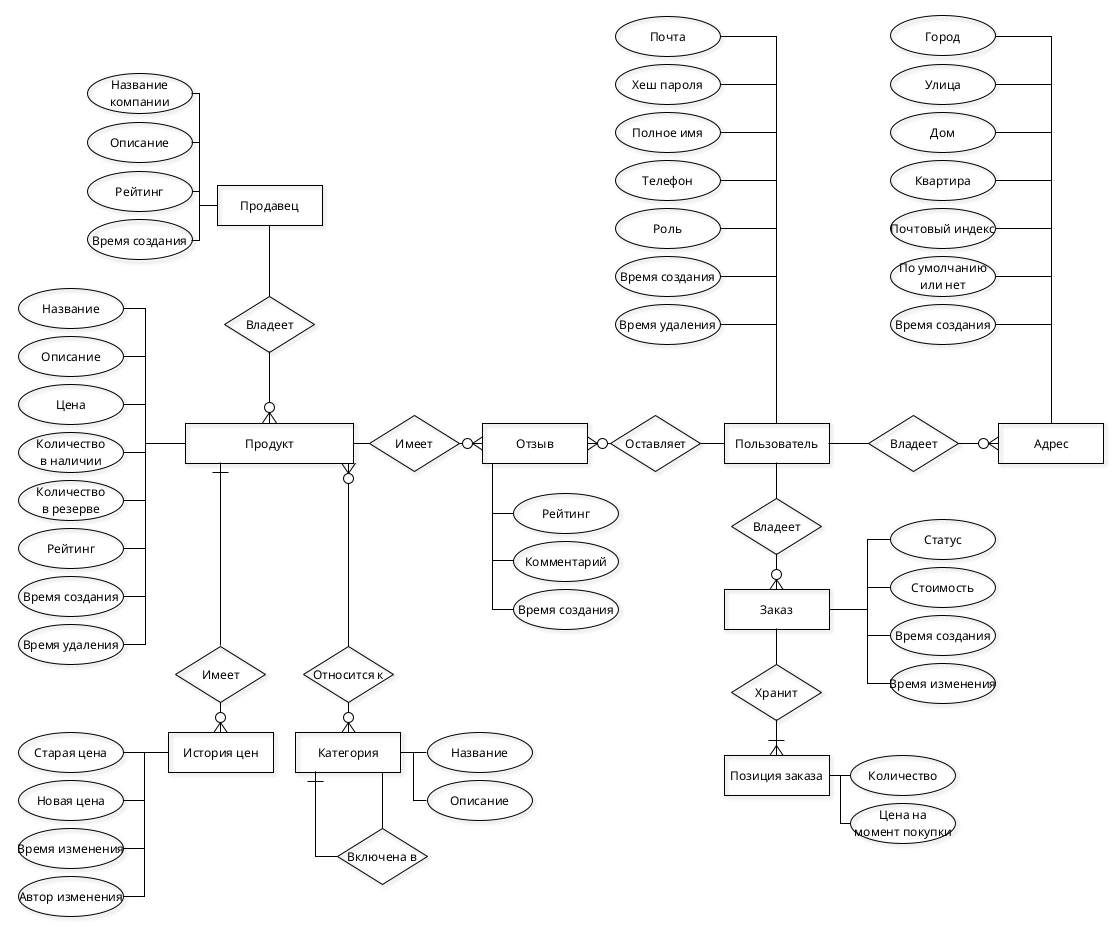
\includegraphics[width=\textwidth]{img/ER_Chen.png}
    \caption{Диаграмма сущность-связь в нотации Чена}
    \label{fig:ER}
\end{figure}

Бизнес-правило <<корзина как черновик заказа>> позволяет не выделять корзину в самостоятельную сущность. Черновик заказа не связан с адресом доставки и продавцом, а при оформлении разделяется на несколько заказов --- по одному на каждого продавца. В момент оформления фиксируется цена товара для соответствующей позиции заказа.

Для контроля доступного остатка товара учитываются общий остаток у продавца и количество товара, находящееся в резерве по оформленным заказам. Доступное для нового заказа количество определяется как разность общего остатка и зарезервированного количества.

Жизненный цикл заказа включает состояния черновика, ожидания оплаты, оплаты, отгрузки, доставки и отмены. При оформлении заказа товар резервируется. При отмене заказа или истечении срока оплаты резерв освобождается. При отгрузке уменьшается общий складской остаток и соответствующее количество в резерве. Отмена заказа допускается до отгрузки.

Для формирования аналитической отчётности необходимы показатели по продавцу за временной интервал: количество заказов, общая выручка, средний чек и наименование самого продаваемого товара.
